\chapter{Big Data} % Main chapter title

\label{Chapterbigdata} % Change X to a consecutive number; for referencing this chapter elsewhere, use \ref{ChapterX}

%----------------------------------------------------------------------------------------
%	SECTION 1
%----------------------------------------------------------------------------------------
%Since the Internet and social networks came up
\section{Introduction}
Over the last decades, the amount of data created has been growing year on year due to Internet and Social Network, consequently under this explosive increase of global data, the term \textit{Big Data} is mainly used to describe enormous dataset. 
Compared with traditional datasets, big data typically includes masses of unstructured data that need more real-time analysis \cite{chen2014big}.

Nowadays, big data related to the service of Internet companies grow rapidly, for instance, Google processes more than 24 petabytes of data per day, or 400 millions of tweets are sent every day \cite{john2014big} however, not only Internet companies deal with Big Data but also traditional research fields such as, transportation, biology, medicine, business activities or even national security are involved in Big Data \cite{lv2017next}.The birth of big data cannot avoid mentioning another current popular term - social networks - and the relation between the two is obvious \cite{lv2017next}. All of this, demonstrates how important is Big Data in today's society.


\section{Definition and features of Big Data}

Big data is an abstract concept, therefore, there exists several different definitions of it, for instance one of them describes the term \textit{Big Data} as the huge volumes of (digital) data that are collected from large variety of sources that are too large, raw, or unstructured for analysis through conventional database techniques \cite{kim2014big}, other definitions focus on the fact that the effort to manage Big Data is higher than traditional approach, for example Chen et al.\cite{chen2014big} define it as, the data that cannot be processed or analyzed using traditional techniques; consequently,not we need to change the way of dealing with Big Data but also, how we apply the new techniques so as to cope with the huge amount of data.
In fact, one of the main benefits of this new approach is that Big Data provides opportunities for discovering new values, helps us to gain an in-depth understanding of the hidden values. 

As a matter of fact, big data has been defined as early as 2001, in this report \cite{laney20013d} Doug Laney defined challenges and opportunities brought about by increased data with a 3V's model, i.e., the increase of Volume, Velocity, and Variety however, nowadays we cannot only define Big Data with the 3V's we need to use the 5 V's: Volume, Velocity, Variety, Value and Veracity \cite{zakir2015big}.

The following is a more detailed explanation of these Big Data features.

\begin{itemize}
\item \textbf{\textit{Volume}.} Over time, systems and humans being are constantly creating new data, resulting in an incredible volume of data.For instance, more than 5 billion individuals are using various mobiles devices \cite{khan2014big} hence, the volume each year is growing more and more.
\item \textbf{\textit{Velocity}.} Velocity means the timeliness of big data, must be rapidly and timely conducted, thus information is flowing at high speed and should be deal with a sensible way.
\item \textbf{\textit{Variety}.} Organized and unorganized information are producing a variety of data types. It is worthing mention that there exist various types of data, which include semi-structured and unstructured data such as audio, video, webpage, and text, as well as traditional structured data.
\item \textbf{\textit{Veracity}.} Veracity includes questions of trust and uncertainty with regards to data and the outcome of analysis of that data, thus,identifying and verifying inconsistent information is significant, to accomplish faithful study. Creating faith in big data is a big challenge to manage even more variety of data is available.
\item \textbf{\textit{Value}.} The main goal of Big Data is to get utility value in terms of analyzing or discovering new features from the original data. 
\end{itemize}

\subsection{Big Data analytic}
Big Data Analytic reflect the challenges of data that are too vast, too unstructured, and too fast moving to be managed by traditional methods. Input to Big Data systems comes from various sources. Traditionally, the largest amount of data were created by business such as paper, audio or photographs records however, nowadays,there exists plenty of emerging sources thank to new technologies, for instance we have millions of big computer networks in different fields which are creating new data in real time, furthermore social networks are a powerful data source, Figure \ref{fig:bigdatasources} shows a briefly view of data sources. 

\begin{figure}[H] %tb
\label{fig:bigdatasources}
	\vspace{0.5cm} \centering 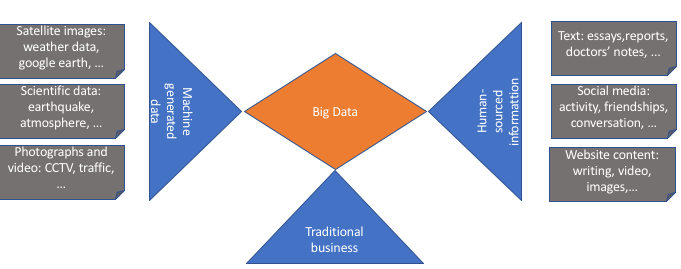
\includegraphics[width=0.95\textwidth]{figures/bigData/BigData_Classification.png}
	\caption{Big Data Sources.}\vspace{0.5cm}
\end{figure}

\subsubsection{Data Types for Big Data}

When we are defining the types of data which are present in Big Data we can sum them up in three types.

\begin{itemize}
\item \textbf{\textit{Structured data}}. Structured Data is any set of data values conforming to a common schema or type \cite{arasu2003extracting}, that is to say, this kind of data refers to information with a high degree of organization, such as sensor data, web log data, financial data (stock-trading data), to sum up, all the data which can be stored in a data base.
\item \textbf{\textit{Semi-structured and complex data}}Semi-structured data is becoming more and more prevalent, Semi-structured data contains semantic tags (some organization) , but does not conform to the structure associated with typical relational databases \cite{buneman1997semistructured}, for instance, emails, XML files, markup languages,etc.
\item \textbf{\textit{Unstructured data}}. Unstructured data has internal structure but is not structured via predefined data models or schema \cite{baars2008management}. This sort of data can be stored in NoSQL data base. Some examples of unstructured data are, text files, data form social mp3,photos, videos, etc.
\end{itemize}


\subsubsection{Technologies}

Big Data is linked to a wide range of technologies whose aims are diverse from collect all the data to and show the results and analyze it. Bellow we describe the most important of these technologies.

\emph{Cloud computing}%\index{Cloud computing}

The National Institute of Standards and Technology (NIST) of the U.S. Department of Commerce defines Cloud computing as \textit{Cloud computing is a model for enabling ubiquitous, convenient, on-demand network access to a shared pool of configurable computing resources (e.g., networks, servers, storage, applications, and services) that can be rapidly provisioned and released with minimal management effort or service provider interaction} \cite{mell2011nist}.
The main objective of cloud computing is to use huge computing and storage resources under concentrated management, consequently both technologies, Big Data and cloud computing, give each other feedback and are growing together. One one hand the development of cloud computing provides  solutions for the storage and processing of big data. On the other hand, the emergence of big data also accelerates the development of cloud computing.

Therefore, Big Data uses cloud computing  as a service, the three most popular cloud paradigms include: Infrastructure as a Service (IaaS), Platform as a Service (PaaS), and Software as a Service (SaaS) \cite{agrawal2010big}.


\emph{Internet of things}%\index{Internet of thing}

The Cluster of European research projects on the Internet of Things (IoT) defines it as \textit{'Things' are active participants in business, information and social processes where they are enabled to interact and communicate among themselves and with the environment by exchanging data and information sensed about the environment, while reacting autonomously to the real and physical world events and influencing it by running processes that trigger actions and create services with or without direct human intervention.}\cite{sundmaeker2010vision}.

Given their inherent nature, IoT has become rapidly in an important Big Data's data source, there exists numerous applications whose data sources are from IoT, Figure \ref{fig:iotbigdata} illustrates the family of applications regarded with  IoT \cite{atzori2010internet}.

\begin{figure}[H] %tb
\label{fig:iotbigdata}
	\vspace{0.5cm} \centering 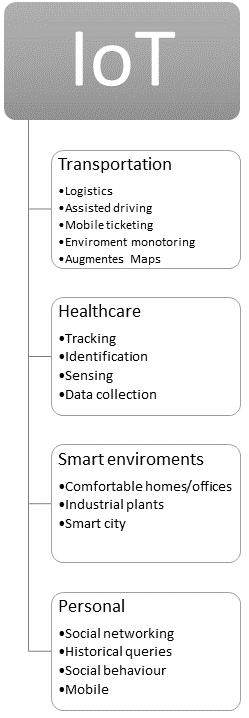
\includegraphics[width=0.30\textwidth,height=0.49\textheight]{figures/bigData/iot.png}
	\caption{Internet of things applications.}\vspace{0.5cm}
\end{figure}


\emph{NoSQL}\index{NoSQL}


Not Only SQL (\textit{NoSQL}), refers to the familiar group of non-relational data management systems. The main feature of this databases is the fact that are not built primarily on tables, and generally do not use SQL for data manipulation. NoSQL database are useful when working with a huge quantity of (un)structured data.

NoSQL systems are distributed, non-relational databases designed for large-scale data storage and for massively-parallel data processing across a large number of commodity servers \cite{moniruzzaman2013nosql}.

Classic relational database management systems (RDBMS) are unable to handle the rapid growth of the data with different (or without) structure of information, and that is the reason why NoSQL databases come up

Han \emph{et al.} \cite{han2011survey} classifies NoSQL databases in three types regard with how it is defined their data model, \textit{key-value} ,\textit{clumn-oriented} and \textit{document}.
\begin{itemize}
    \item \textbf{\textit{Key-value}}. These database store items as alpha-numeric identifiers (keys) and associate values in simple. The values may be various from simple text strings to  more complex like lists or sets. Data searches can usually only be performed against keys, not values, and are limited to exact matches. Examples of this type of database are, Redis \cite{carlson2013redis},  Tokyo Cabinet-Tokyo Tyrant \cite{cattell2011scalable} or Scalaris \cite{leavitt2010will}
    \item \textbf{\textit{Column-oriented}}. The data model of this kind of database is defined as rows and columns, although we could think this database share same model as RDBMS this not really, because Column-oriented databases have an architecture with data compression, shared-nothing, massively parallel processing. As Column-oriented databases we could highlight the following, HBase \cite{george2011hbase}, HadoopDB \cite{abouzeid2009hadoopdb}, Apache Cassandra \cite{dede2013evaluation} or Google's Bigtable \cite{chang2008bigtable}.
    \item \textbf{\textit{Document}}. Document database and Key-value share very similar structure however, the Value of document database is semantic, and is stored in JSON or XML format therefore, document stores support more complex data than the key-value stores. Documents can be any type of traditional document such as, articles, Microsoft Words, etc or other type such as, register, list, etc. Some instances of document database are, MongoDB \cite{banker2011mongodb} or CouchDB \cite{provost2013data}.
\end{itemize}

\emph{Hadoop and MapReduce}\index{MapReduce}

In the early years of 2000 Google started off the development of a distributed file system called \textit{Google File System} (GFS) \cite{ghemawat2003google} whose main goal was to tackle with the issue of managing enormous amount of data using computer clusters. Only one year later, \textit{Apache} created the project \textit{Hadoop} which its components, \textit{MapReduce} and \textit{Hadoop Distributed File System} (HDFS) are inspired by GFS.

Hadoop is an Apache project therefore, all components are available via the Apache open source license. It is worth mentioning that Yahoo! has developed and contributed to 80\% of the core of Hadoop (HDFS and MapReduce) \cite{shvachko2010hadoop}.

\emph{HDFS} is a distributed file system designed to run on commodity hardware.  HDFS not only  stores application data but also metadata, this metadata are stored on dedicated server, called the NameNode. Application data are stored on other servers called DataNodes. All servers are fully connected and communicate with each other using TCP-based protocols.

HDFS has a master/worker architecture. An HDFS cluster consists of a single NameNode, a master server that manages the file system namespace and regulates access to files by clients.
In addition, there are a number of DataNodes, usually one per node in the cluster, which
manage storage attached to the nodes that they run on. HDFS exposes a file system
namespace and allows user data to be stored in files. Internally, a file is split into one or more blocks and these blocks are stored in a set of DataNodes. The NameNode executes file
system namespace operations like any other file system, such as, list, copy, delete and so on. It
also determines the mapping of blocks to DataNodes. The DataNodes are responsible for
serving read and write requests from the file system’s clients. The DataNodes also perform
block creation, deletion, and replication upon instruction from the NameNode.

\emph{Spark}\index{Spark}
\subsubsection{Big data generation and acquisition}
One of the drawback of Big Data is that is not always useful owing to data may have inconsistent information. The actual challenge of big data is not in collecting it, but in managing it as well as making sense of it.

There are a myriad of analytic techniques that could be employed when dealing with a Big Data challenge. Which ones are used depends on the type of data being analyzed, as well as the technology available to you and the questions you are trying to solve. 
%In order to identify data as Big Data should be analyzed from different dimensions
%Big Data analysis allows to extract information from these data. Many software solutions around the Apache Hadoop project are solving encountered problems through this and other complementary projects.

%Ideally, these advances allow to easy the access o Big Data, bringing it closer to SMEs, but the rapid development of these technologies and the lack of qualified professionals currently make SMEs have difficulties to take advantage of those technologies. The building of framewoks aimed at Big Data analysis, which allow reusing of solutions and algorithms, will make these technologies more accessible.
%Business Intelligence or BI comprises a set of strategies and tools focused on managing and creating knowledge through the analysis of existing data in an organization. BI tools are based on the use of an information system that is built with different data from production process, with information related to the business and economic data. This set of tools and methodologies have in common information accessibility, decision-making support, and focus to the end user.
%The full interconnection between the results of Big Data analysis and BI has to deal with the problem of establishing the relationship between these results and the data models used by technical analysis and dashboards of BI applications. The automatic interpretation of results f the Big Data analysis, by exposing their semantics and preserving the context of how they have been produced, are some of the challenges to be addressed when trying to add these results to business processes.
%In this scenario, the concept of Smart Data emerges. It is defined as the result of the process of analysis performed to extract relevant information and knowledge from Big Data, including context information and using a standardized format. By context we mean all the relevant (meta) information to interpret the analysis results. This will lead to the enforceability of these results and thus facilitating their interpretation, the easy integration with other structured data, the integration of the Big Data analysis system with the BI systems, the interconnection (in a standardized way, at a lower cost and a higher accuracy and reliability) of third parties algorithms and services, etc.
